\chapter{Kravspecifikation}

\section{Indledning}
Kravspecifikationen vil beskrive, ud fra en række modeller, hvordan EKG-systemet fungerer. Helt generelt er EKG-måling en simpelt metode, til at måle hjertets elektriske aktivitet via elektroder, som registrerer elektriske impulser, placeret på huden. Ud fra disse impulser dannes en graf, som benyttes til at analysere hjertets funktionalitet ud fra P-, Q-, R-, S- og T-takkerne, og dermed konkludere om den pågældende patient har et raskt eller sygt hjerte, samt hvilken sygdom der er tale om.

\section{Funktionelle krav}
De funktionelle krav vil nedenstående beskrives ud fra Aktør-kontekstdiagram, aktørbeskrivelse, Use Cases samt Use Case diagram. 

\subsection{Aktør-kontekstdiagram}

\begin{figure}[htb]
	\centering
	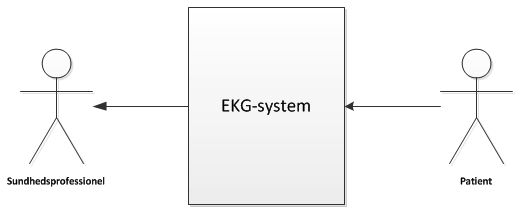
\includegraphics[width=1\textwidth]{Figurer/Snip20150226_1}
	\caption{Aktør-kontekstdiagram}
	\label{fig:aktoerbeskrivelse}
\end{figure}

Patient kobles op med elektroderne fra EKG-systemet (jf. use case 1). Patientens data bliver opsamlet af EKG-systemet, ud fra disse data danner EKG-systemet en graf. Grafen kan derefter valideres og analyseres af den sundhedsprofessionelle. 

\subsection{Aktørbeskrivelse}

\begin{table}[H]
\begin{tabularx}{\textwidth}{l l X}
    \toprule
     Aktørnavn  & Type      & Beskrivelse \\ \midrule
     Sundhedsprofessionelle   & Primær    & Det er den sundhedsproffesionelle, der ønsker at foretage EKG-målinger samt analysere på EKG-grafen.\\ 						  									  \addlinespace[2mm]
     Patienten & Sekundær  & Patienten sender elektroniske signaler til EKG-systemet, via elektroder, som er placeret på patientens krop\\                                                                                                                                                                            
   
     \bottomrule                                                                                                                   
    \end{tabularx}
    \caption {Aktørbeskrivelse}
    \label{tab:aktoerbeskrivelse}
	
\end{table}

\subsection{Use Cases}

\begin{table}[H] % UC1 % 
    \begin{tabularx}{\textwidth}{l X}
    \toprule 
    \multicolumn{2}{c}{\begin{large}\textbf{Use Case 1}\end{large}}
 \\ \midrule \addlinespace[1mm]                                                                                                                                                        
     Navn:                  &  Vis EKG. \\ \addlinespace[1mm]                                                                                                                                                       
     Use Case ID:           & 1                                                                                                                                                                                                                                                                                                                                                                                                                                                                                                                                                                                                                         \\ \addlinespace[1mm]                                                                                                                                                       
     Samtidige forekomster: & 1                                                                                                                                                                                                                                                                                                                                                                                                                                                                                                                                                                                                                         \\ \addlinespace[1mm]                                                                                                                                                       
     Primær aktør:          &	Sundhedsprofessionelle.                                                                                                                                                                                                                                                                                                                                                                                                                                                                                                                                                                                                                 \\ \addlinespace[1mm] 
     Sekundær aktør:        &	Patienten                                                                                                                                                                                                                                                                                                                                                                                                                                                                                                                                                                                                                 \\ \addlinespace[1mm]  		                                                                                                                                                      
     Initialisere:          & 	Den sundhedsprofessionelle ønsker at få vist et EKG-signal over patienten.
		 \\ \addlinespace[1mm]                                                                                                                                                                                                                                                                                                             
     Forudsætninger:        & 	EKG-elektroder er koblet rigtigt op på patienten ud fra afledning II
     \begin{itemize}
     	\item Rød(+) på venstre ben
     	\item Sort(-) på højre arm
     	\item Grøn på venstre arm
     \end{itemize}
		Samt EKG-systemet er tændt og klar til måling.                                                                                                                                                                                                                                                                                                                                                                                                                                                                                                                                                                           \\ \addlinespace[1mm]                                                                                                                                                       
     Resultat:              & 	Den sundhedsprofessionelle kan ud fra EKG-dataerne se en graf.                                                                                                                                                                                                                                                                                                                                                                                                                                                                                                                                                   \\ \midrule \addlinespace[1mm]                                                                                                                                                       
     Hovedforløb:           &  \begin{enumerate}
     						   \item Den sundhedsprofessionelle vælger indstillinger
\newline						[Extension 2a: Den sundhedsprofessioneller er tilfreds med default-indstillingerne]
     						   \item Målingen startes ved at trykke på "Start"
		   				   	   \item EKG-dataerne illustreres på en graf
     						   \end{enumerate}
\\ \midrule 
 	Undtagelser:           & \textit{Extensions:}
\newline					 2a: Der blev ikke ændret i indstillingerne. Målingen foretages med default indstillinger 
\\ \bottomrule
    \end{tabularx}
    \caption {Fullydressed Use Case beskrivelse af UC1.}
    \label{tab:UC1}
\end{table}




\begin{table}[H] % UC2 % 
    \begin{tabularx}{\textwidth}{l X}
    \toprule 
    \multicolumn{2}{c}{\begin{large}\textbf{Use Case 2}\end{large}}
 \\ \midrule \addlinespace[1mm]                                                                                                                                                        
     Navn:                  &  Evaluer EKG i forhold til HRV. \\ \addlinespace[1mm]                                                                                                                                                       
     Use Case ID:           & 2                                                                                                                                                                                                                                                                                                                                                                                                                                                                                                                                                                                                                         \\ \addlinespace[1mm]                                                                                                                                                       
     Samtidige forekomster: & 1                                                                                                                                                                                                                                                                                                                                                                                                                                                                                                                                                                                                                         \\ \addlinespace[1mm]                                                                                                                                                       
     Primær aktør:          &	Sundhedsprofessionelle.                                                                                                                                                                                                                                                                                                                                                                                                                                                                                                                                                                                                                 \\ \addlinespace[1mm] 	                                                                                                                                                      
     Initialisere:          & 	At kunne evaluere variationen i længden af RR-intervaller.
		 \\ \addlinespace[1mm]                                                                                                                                                                                                                                                                                                             
     Forudsætninger:        & 	Use Case 1 er gennemført.                                                                                                                                                                                                                                                                                                                                                                                                                                                                                                                                                                           \\ \addlinespace[1mm]                                                                                                                                                       
     Resultat:              & 	HRV kan ses ud fra grafen.                                                                                                                                                                                                                                                                                                                                                                                                                                                                                                                          \\ \midrule \addlinespace[1mm]                                                                                                                                                       
     Hovedforløb:           &  \begin{enumerate}
     						   \item Den sundhedsprofessionelle måler længden mellem RR-intervallerne.
     						   \item Den sundhedsprofessionelle analysere målingerne
     						   \item HRV er identificeret
\newline						[Extensions 3a: HRV er ikke identificerbart]
     						   \end{enumerate}
\\ \midrule 
 	Undtagelser:           & \textit{Extensions:}
\newline					 3a: Det er er ikke mulig at analysere HRV ud fra grafen. Use Case 1 gentages, ny graf analyseres.
\\ \bottomrule
    \end{tabularx}
    \caption {Fullydressed Use Case beskrivelse af UC2.}
    \label{tab:UC2}
\end{table}

\subsection{Use case-diagram}

\begin{figure}[htb]
	\centering
	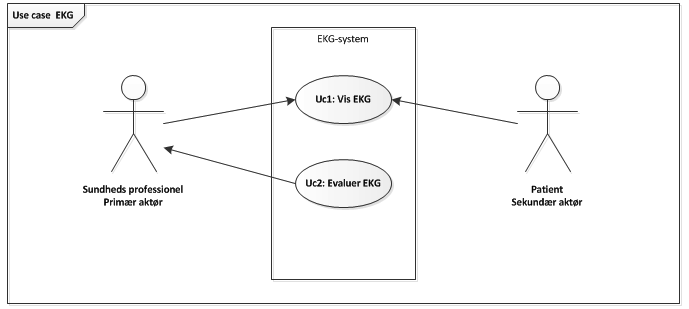
\includegraphics[width=1\textwidth]{Figurer/Snip20150226_2}
	\caption{Use case-diagram}
	\label{fig:Use Cases}
\end{figure}

Den sekundære aktør, Patienten, er koblet op til elektroderne og EKG-systemet, som på kommando af den primære aktør, den sundhedsprofesionelle, danner en graf (Uc1: Vis EKG). Denne graf kan den sundhedsprofessionelle efterfølgende evaluere (Uc2: Evaluer EKG).

\section{Ikke-funktionelle krav}
De ikke-funktionelle krav er udarbejdet ved brug af (F)URPS+. De er alle prioriteret ved MuSCoW metoden - Must (skal være med), Should (bør være med, hvis muligt), Could (kunne have med, hvis det ikke influerer på andet), Won't/Would (ikke med nu, men med i fremtidige opdateringer). 

\subsection{(F)URPS+}
MoSCoW er angivet i parentes med hhv. M, S, C eller W.

\textbf{Usability}
\begin{itemize}
	\item (M) Den sundhedsprofessionelle skal kunne starte en default-måling maksimalt 20 sek. efter opstart af programmet
	\item (M) Den sundhedsprofessionelle skal have mulighed for at ændre tidsintervallet før målingerne foretages
	\item (M) Interfacet skal indeholde en "start"-knap til at igangsætte målingerne
	\item (M) Programmet stopper automatisk efter det valgte tidsinterval
	\item (C) Programmet kan indeholde "pause/stop-knap"
	\item (S) Interfacet bør anvendes på en touch-skærm. Dette gør den nemmere at rengøre og simplere at anvende
	\item (S) Der bør kræves et login i form af patientens cpr-nummer inden opstart af programmet
\end{itemize}

\textbf{Reliability}
\begin{itemize}
	\item (S) Softwaren skal opdateres to gange årligt
	\item (M) Systemet skal have en effektiv MTBF (Mean Time Between Failure) på 43.680 timer og en MTTR (Mean Time To Restore) på 48 timer.
	\item  
				\begin{align}
					Availability = \frac{MTBF}{MTBF+MTTR} = \frac{43.680}{43.680+48} = 0,998 = 99,8 \%
				\end{align}

\end{itemize}

\textbf{Performance}
\begin{itemize}
	\item (M) Der skal vises en EKG-graf i interfacet, hvor spænding vises op af y-aksen (-1V – 1V) og tiden på x-aksen
	\item (M) Grafen skal have major gridlines hver 0,5 mV og minor gridlines hver 0,1 mV på y-aksen og major gridlines hver 200 ms. og minor gridlines hver 40 ms. på x-aksen
	\item (M) Grafen skal være scrollbar på x-aksen, så den sundhedsprofessionelle selv ved brug af musen kan vælge det udsnit af grafen der skal vises mere detaljeret
	\item (S) Det er ønskeligt hvis en 1 mV signal-tak kan vises i starten af grafen som reference for det målte EKG-signal
	\item (M) Skal tage en sample over et brugerbestemt interval, hvor frekvensen  er tilpasset målingerne, således at grafen er analyserbar
\end{itemize}

\textbf{Supportability}
\begin{itemize}
	\item (M) Softwaren udarbejdes i Visual Studio
	\item (M) Softwaren er opbygget af trelagsmodellen
	\item (C) Systemet skal selv kunne søge efter opdateringer. Den skal selv kunne opdateres såfremt det ikke påvirker målingerne
\end{itemize}














